% !TeX spellcheck = en_US
\section{Background}\label{sec:background}

\subsection{Deep learning}
\gls{dl} is a set of machine learning techniques that aim at learning representations of data with several levels of abstraction by using models with multiple processing layers \cite{DL2}. Most of the deep learning architectures are based on \glspl{ann} due to their hierarchical property \cite{DL1} \cite{DBLP:DEEPSISR}.

These set of methods have been applied in multiple fields such as speech recognition, computer vision, genomics or natural language processing bringing important breakthroughs in many research areas. More specifically, \glspl{cnn} have had a relevant impact in the field of computer vision since they have achieved superior results in tasks like object recognition, video analysis, image classification or image restoration.

\subsection{Convolutional Neural Networks}
\gls{cnn} is a class of deep neural networks that has recently shown increasing popularity due to its success in natural language processing and computer vision fields.

\glspl{cnn} are different from others \glspl{ann} in the sense that former uses the convolution operation instead of matrix multiplication to propagate the data. This convolution operation is applied in the hidden layers of the \glspl{cnn} by convolutional layers. Before introducing the convolutional layers, we present the concepts of convolution, padding and stride.

\paragraph{Convolution.} 

A \textbf{convolution} is a mathematical operation, usually denoted by the asterisk ($\ast$) operator, that transforms two functions, $f$ and $g$, in a third one, $f\ast g$, that represents the amount of overlap of $g$ as it is shifted over $f$.

In image processing, an image is convolved with a convolution matrix, or kernel, by adding an image data point to its neighbors, that are weighted by the kernel. The kernel is used as a sliding window that traverses the image being processed in order to compute all the result values. Figure \ref{fig:convolution} shows a graphical representation of the described process.

\begin{figure}
	\centering
	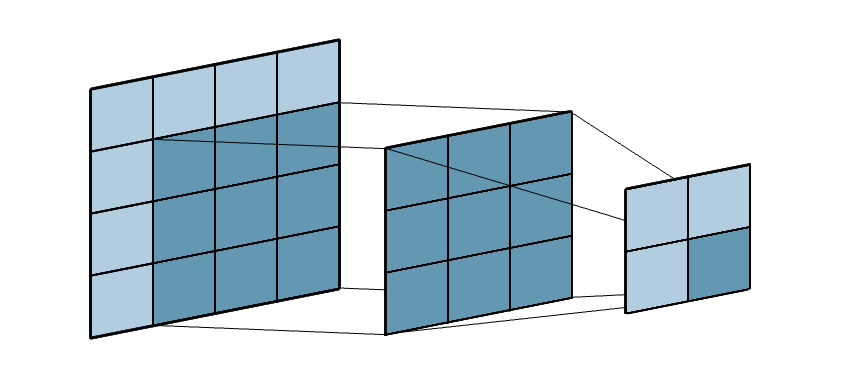
\includegraphics[width=0.5\textwidth]{images/convolution.png}
	\caption{Convolution of a $4\times4$ matrix with a $3\times3$ matrix resulting in a $2\times2$ matrix.}
	\label{fig:convolution}
\end{figure}

\paragraph{Padding.}
As shown in Figure \ref{fig:convolution}, one of the effects observed when convolving an image with a kernel is that the resulting matrix has a smaller size than the input image. \textbf{Padding} solves this issue by adding extra values to the boundary of the original image so that its size is effectively increased and the result of the convolution has the same size as the original input.

In convolution, when there is a need of increasing the size of the input data, zero-padding is typically used, meaning that the image is padded evenly by adding rows and columns of zeroes. If the right amount of zero-padding is used, this operation is known as \textbf{same} padding, since after the convolution, the output will keep the same spatial dimensions as its input. Figure \ref{fig:padding} shows an example of the application of same padding.

\begin{figure}
	\centering
	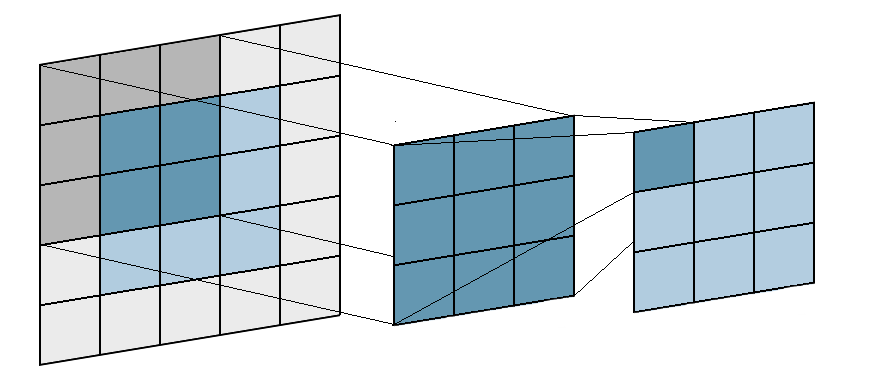
\includegraphics[width=0.5\textwidth]{images/padding.png}
	\caption{Convolution with same padding. In the image, zero-padding is applied to a $3\times3$ matrix in order to have a $5\times5$ matrix as an input. The resulting input matrix is convolved with a $2\times2$ kernel producing a $3\times3$ output matrix.}
	\label{fig:padding}
\end{figure}

On the other hand, when there is no padding applied to the input of the convolution, the kernel always stays at a valid position within the input matrix, producing that the output size shrinks depending on the kernel size. For this reason, this kind of padding can be called \textbf{valid} padding or no-padding. Figure \ref{fig:convolution} shows this behavior.

\paragraph{Stride.}
When an image is convolved with a kernel, the kernel is shifted over the image in order to compute each cell value of the output matrix. In figures \ref{fig:convolution} and \ref{fig:padding}, we slide the kernel 1 cell at a time, however, the number of pixels traversed per slide can be different that 1. This number is called \textbf{stride}, and it represents the number of cells that the kernel matrix is shifted over the input matrix in order to compute the next output cell value.

\subsubsection*{Convolutional layers}
Convolutional layers take matrices with dimensions $(w_1, h_1, c_1)$ that represent input images with width $w_1$, height $h_1$ and $c_1$ channels. This matrices are convolved with $k$ filters of size $f$, producing an output matrix with dimensions $(w_2, h_2, c_2)$, with:

\begin{itemize}
	\item $w_2 = \frac{w_1 - f + 2p}{s} + 1$
	\item $h_2 = \frac{h_2 - f + 2p}{s} + 1$
	\item $c_2 = k$
\end{itemize}
where $p$ is the the amount of zero-padding used and $s$ is the value of the stride \cite{STANFORD}. It is worth noting that the third dimension of the output is given by the amount of filter used, no matter what the input's third dimension is.

\subsubsection*{Architecture of CNNs}
The architecture of a \gls{cnn} varies depending on the task being performed, although all architectures typically share:
\begin{itemize}
	\item An \textbf{input layer} that is a tensor with shape 
	$(n, r, c, d)$, where $n$ is the number of images to be processed, $r$ is the number of rows of pixels or image height, $c$ is the number of columns of pixels or image width, and $d$ is the image depth or number of channels.
	\item Multiple \textbf{hidden layers}, usually convolutional layers, that convolve their input with a set of $k$ filters, producing a set of filtered images as a result that will be used as the input of the next layer.
	\item \textbf{Activation layers} that apply an activation function to the result of the hidden layer. In \gls{cnn}, the most commonly used activation function is \gls{relu}, since it has demonstrated to make convergence faster \cite{RELU}.
\end{itemize}

Depending on the task being carried out, the architecture can also present:
\begin{itemize}
	\item \textbf{Pooling layers}, that shrink the image stack produced by the convolution layers. These typically consist of filters of a given size that are used to downsize the resulting matrix of the convolution layer. There are different types of pooling layers depending on the used pooling function. These usually are: max pooling and average pooling.
	\item \textbf{Fully connected layers}, that will compute the class scores. Each neuron in these layers is connected to all the outputs of the previous layer.
\end{itemize}

\subsection{Single image super-resolution}

\gls{sisr} is a low-level computer vision task that aims at obtaining a \gls{hr} image from an input \gls{lr} image. This problem can be modeled as follows:
$$y = \Phi(x, \theta_\eta)$$
where $y$ is the \gls{lr} image we want to super-resolve, $x$ is the original \gls{hr} image, and $\Phi(x, \theta_\eta)$ denotes the application of a degradation function $\Phi$ to $x$ using the degradation parameters $\theta_\eta$ \cite{DBLP:SISR}. 

Since this degradation process is not known and can be affected by multiple factors such as noise or blur, we can also model the \gls{sisr} problem as follows:

$$y = (x\otimes k)\downarrow_s + n$$

where $(x\otimes k)$ denotes a convolution of the original \gls{hr} image with a blurry kernel $k$, $\downarrow_s$ denotes a downsampling operation with scale factor $s$ and $n$ represents the independent noise term.

\gls{sisr} aims at recovering an approximation of $x$ given given the image $y$, however, it is an ill-posed problem due to the fact that a given \gls{lr} image can correspond to multiple \gls{hr} solutions. \cite{DBLP:DEEPSISR}.

\subsection{Image denoising}
Image denoising or noise reduction is as well a low-level computer vision task that aims at removing the noise from a given image. 

Noise is a random signal in digital images that destroy part of the image information by altering the pixel values. This signals are typically produced by the sensors or electronic circuitry used to obtain the images.

There are multiple types of image noise, such as Gaussian noise, salt-and-pepper noise, speckle noise, quantization noise, Poisson noise, etc. \cite{NOISE}.

We introduce the 4 types of noises we have selected to perform the experiments, namely Gaussian noise, Poisson noise, salt-and-pepper noise and uniform noise. \

\paragraph{Gaussian noise}
Gaussian noise, also called electronic noise, is a type of noise caused by natural sources such as the illumination or the temperature of the sensor. This noise can be modeled as an additive matrix whose values are independent and identically distributed and follow a normal distribution with mean $\mu$ and standard deviation $\sigma$.

\paragraph{Poisson noise}
Poisson noise or shot noise arises because of the discrete nature of the electric charge and it's the dominant noise in the darker parts of the image. Shot noise follows a Poisson distribution.

Is worth mentioning that, apart from the followed distribution, the fundamental difference between Gaussian noise and Poisson noise is that Gaussian noise is additive and Poisson noise is signal dependent. As a result, Poisson noise does not approximate to a Gaussian distribution at low intensity levels.

\paragraph{Salt-and-pepper noise}
Salt-and-pepper noise or impulse value noise is a type of noise that, unlike Gaussian and Poisson noise, completely destroys the information held by part of the image. 

This noise is seen it data transmission and it replaces the corrupted pixels by the minimum or maximum possible value that the pixel can have. In 8-bits images, the minimum value corresponds to 0 and the maximum value, to 255.

The amount of salt-and-pepper noise that a image has is known as noise ratio. An image with a noise ratio of 0 has no salt-and-pepper noise, whereas an image with a noise ratio of 1 has all its pixels affected by the noise.

\paragraph{Uniform noise}
Uniform noise or quantization is typically caused by the quantization process when converting analog to digital images and it follows an uniform distribution. 

Like salt-and-pepper noise, uniform noise completely destroys the information of part of the image. The amount of uniform noise hat an image has is also described with the mentioned concept of noise ratio.

